%%%%%%%%%%%%%%%%%%%%%%%%%%%%%%%%%%%%%%%%%
% Short Sectioned Assignment
% LaTeX Template
% Version 1.0 (5/5/12)
%
% This template has been downloaded from:
% http://www.LaTeXTemplates.com
%
% Original author:
% Frits Wenneker (http://www.howtotex.com)
%
% License:
% CC BY-NC-SA 3.0 (http://creativecommons.org/licenses/by-nc-sa/3.0/)
%
%%%%%%%%%%%%%%%%%%%%%%%%%%%%%%%%%%%%%%%%%

%----------------------------------------------------------------------------
%	PACKAGES AND OTHER DOCUMENT CONFIGURATIONS
%----------------------------------------------------------------------------

\documentclass[paper=a4, fontsize=11pt]{scrartcl} % A4 paper and 11pt font size

\usepackage[T1]{fontenc} % Use 8-bit encoding that has 256 glyphs
\usepackage{fourier} % Use the Adobe Utopia font for the document - comment this line to return to the LaTeX default
\usepackage[english]{babel} % English language/hyphenation
\usepackage{amsmath,amsfonts,amsthm} % Math packages

\usepackage{graphicx} % Used for including graphics
\usepackage{caption}
\usepackage{subcaption}

\usepackage{sectsty} % Allows customizing section commands
\allsectionsfont{\centering \normalfont\scshape} % Make all sections centered, the default font and small caps

\usepackage{fancyhdr} % Custom headers and footers
\usepackage{cite}
\bibliographystyle{plain}
\pagestyle{fancyplain} % Makes all pages in the document conform to the custom headers and footers
\fancyhead{} % No page header - if you want one, create it in the same way as the footers below
\fancyfoot[L]{} % Empty left footer
\fancyfoot[C]{} % Empty center footer
\fancyfoot[R]{\thepage} % Page numbering for right footer
\renewcommand{\headrulewidth}{0pt} % Remove header underlines
\renewcommand{\footrulewidth}{0pt} % Remove footer underlines
\setlength{\headheight}{13.6pt} % Customize the height of the header

\numberwithin{equation}{section} % Number equations within sections (i.e. 1.1, 1.2, 2.1, 2.2 instead of 1, 2, 3, 4)
\numberwithin{figure}{section} % Number figures within sections (i.e. 1.1, 1.2, 2.1, 2.2 instead of 1, 2, 3, 4)
\numberwithin{table}{section} % Number tables within sections (i.e. 1.1, 1.2, 2.1, 2.2 instead of 1, 2, 3, 4)

\setlength\parindent{0pt} % Removes all indentation from paragraphs - comment this line for an assignment with lots of text

%----------------------------------------------------------------------------
%	TITLE SECTION
%----------------------------------------------------------------------------

\newcommand{\horrule}[1]{\rule{\linewidth}{#1}} % Create horizontal rule command with 1 argument of height

\title{
\normalfont \normalsize
\textsc{King Abdullah University of Science and Technology\\
        Division of Mathematical and Computer Sciences and Engineering\\
        Design and Analysis of Algorithms} \\ [25pt] % Your university, school and/or department name(s)
\horrule{0.5pt} \\[0.4cm] % Thin top horizontal rule
\Large Midterm Project Report\\
\huge Diverse Approaches to Exact Pattern Matching
\horrule{2pt} \\[0.5cm] % Thick bottom horizontal rule
}

\author{Affara, Lama\\
        Almansour, Durrah\\
        Al-Shedivat, Maruan\\
        Chen, Gui\\
        Fujii, Chisato\\
        Rapakoulia, Trisevgeni}


\date{\normalsize\today} % Today's date or a custom date


\begin{document}
\begin{titlepage}
\maketitle
\thispagestyle{empty}
\clearpage
\end{titlepage}

%----------------------------------------------------------------------------
%    INTRODUCTION
%----------------------------------------------------------------------------

\section{Introduction}
Write introduction here...

\section{Boyre-Moore Algorithm}
Boyre Moore algorithm \cite{bm_fast} searches for all the occurrences of the pattern in the text. It is in some way similar to the naive search algorithm. Initially, it aligns the first character in P with the first character in T. The algorithm then compares characters between P and T sequentially from right to left. Once a mismatch occurs, a shift rule is applied thus moving the pattern by $s\ge 1$. The algorithm is basically divided into two stages: preprocessing and searching. There are two different preprocessing approaches in the literature: Bad Character Rule and Good Suffix Tree \cite{bm_tbc}. We decided to choose the Bad Character rule due to its simplicity and applicability to our dataset. In the following sections, we describe the two stages of the algorithm.

\subsection{Preprocessing Stage}
In the preprocessing stage, the algorithm makes use of the alphabet $\Sigma$ and the pattern P. A two dimensional table D is constructed by processing the pattern according to the available alphabet. D is of size $k\times|\Sigma|$ where for each mismatch index in P, the position of rightmost occurrence of a character in $\Sigma$ is stored. Figure \ref{fig:table} shows an example of the table stored by processing the pattern GCAGAGAG based on the DNA alphabet=\{A,C,G,T\}. Starting from the last row corresponding to a mismatch occurring at position i=k in P, i=8 for this example, the algorithm scans P to find the rightmost index of the given character. In the below example, the last occurrence of A before position 8 is 7, G is 6, C is 2, and T is 0. It is important to note here that if a character does not exist in the pattern, its position in the table is always 0. Now, the algorithm iterates from i=k to 1. If the mismatch occurs in position i-1, the algorithm updates only the value for the specific character placed in this position, A for this example, and all the other values remain the same as D[i,x]. The last occurrence of A before position 7 is 5, while G, C, and T stay the same.

\begin{figure}[h!]
\centering
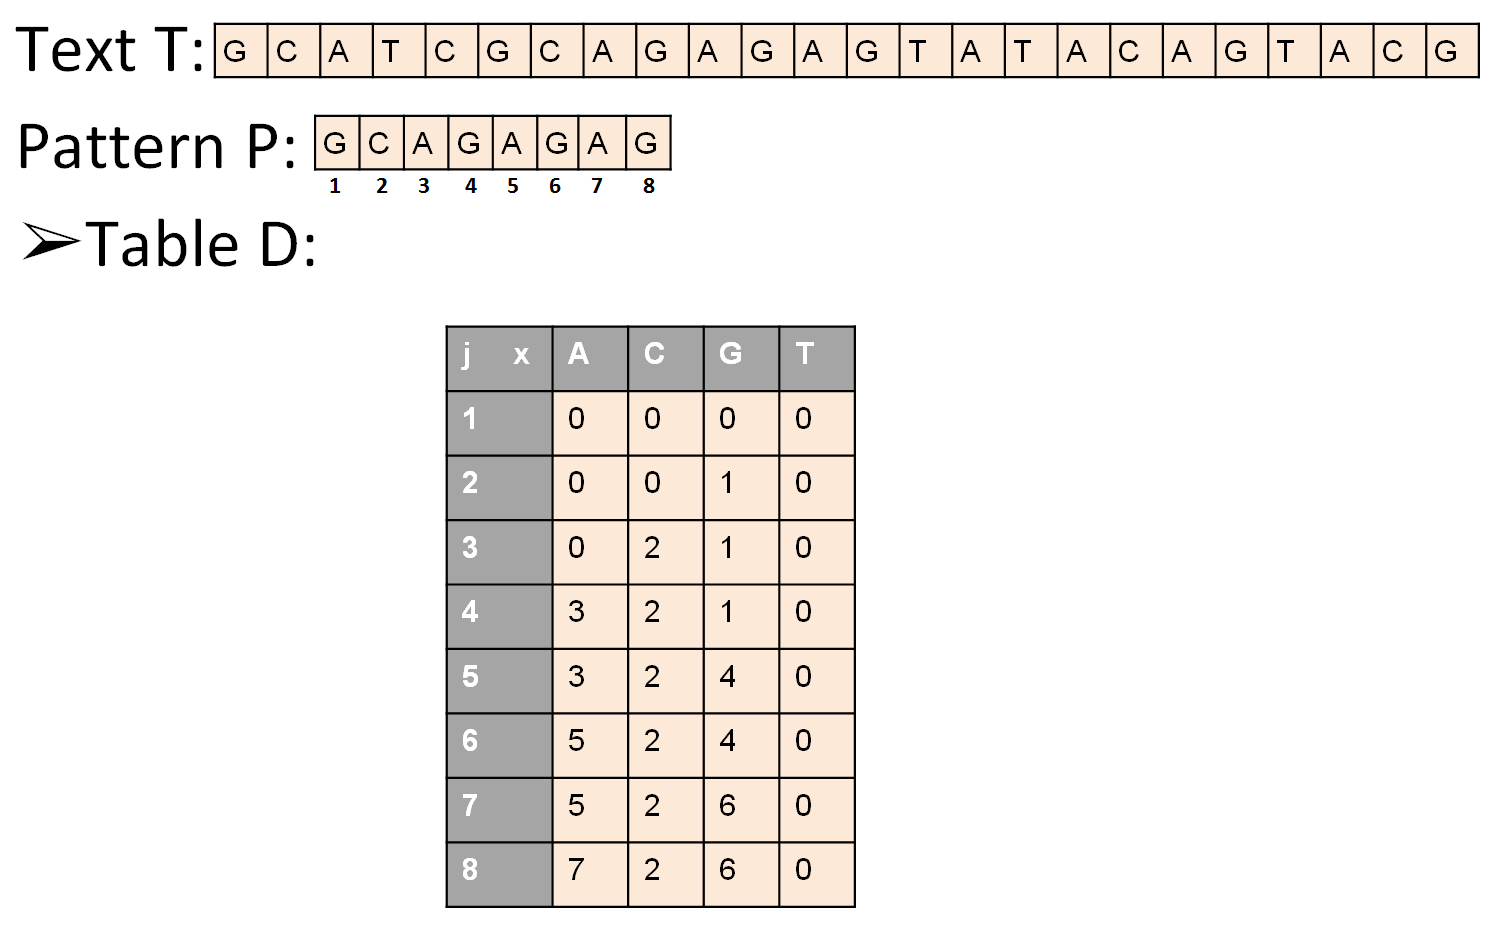
\includegraphics[width=0.8\textwidth]{figures/Example_Table.png}
\caption{Table of preprocessing phase}
\label{fig:table}
\end{figure}

\subsection{Searching Phase}
In the searching phase, the algorithm needs shift the pattern and sequentially match it with the aligned text. Starting from the rightmost character in P, the algorithm checks the aligned character in T. If the pair of characters are matching, it sequentially continues the check to the next left character. If a mismatch occurs at position j in P, the algorithm needs to shift P according to the mismatched character in the text. For example, if at position j, the text contains a character that is not found in P, the pattern should be shifted by j. However, if the mismatched character is found in P, the pattern should be shifted by j-i, where i corresponds to the rightmost occurrence of this character in P. The index i of the last occurrence is retrieved from table D and i=D[j,x] where x is the character in the text. Figure \ref{fig:search} shows the searching phase for the example shown in the previous section.

\begin{figure}[h!]
\centering
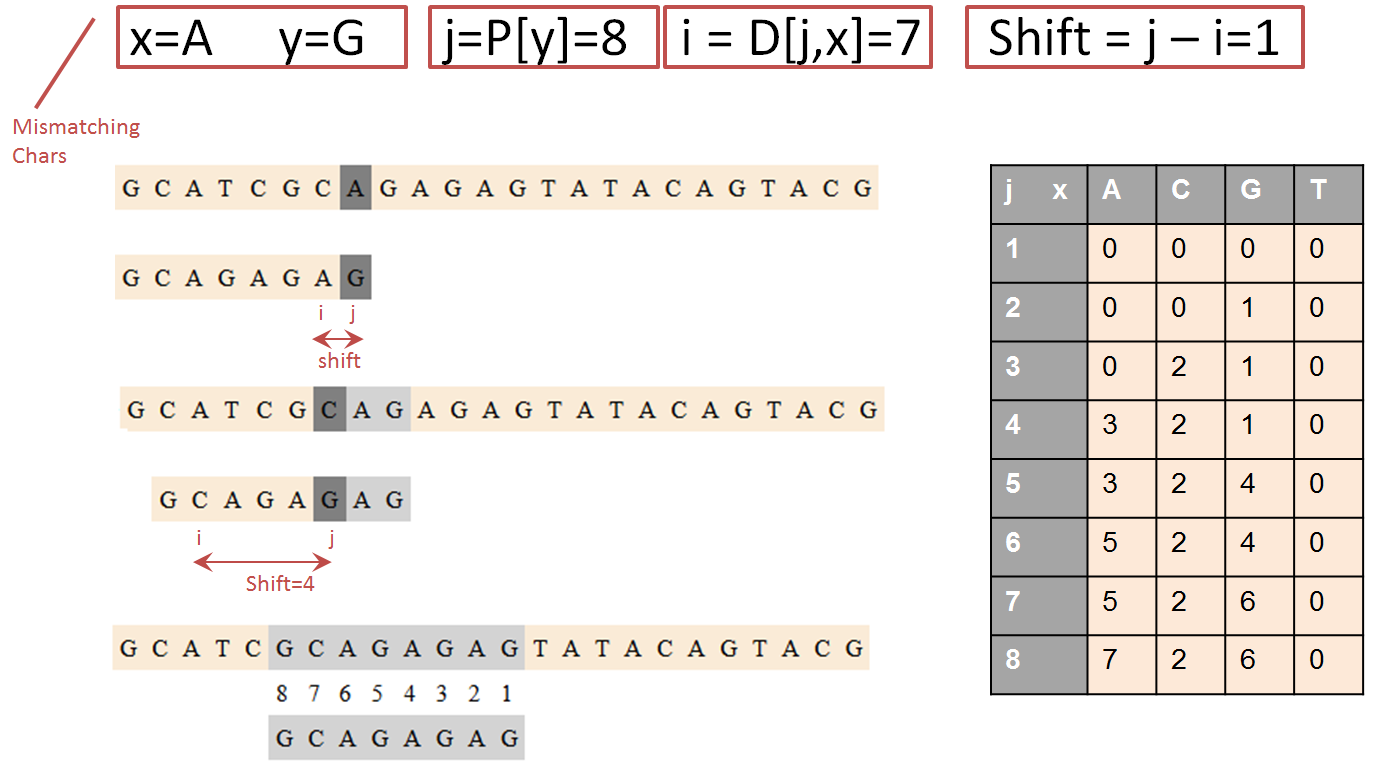
\includegraphics[width=0.8\textwidth]{figures/searching_phase.png}
\caption{Searching Phase}
\label{fig:search}
\end{figure}

\subsection{complexity}

\newpage
\section{Aho-Corasick algorithm}
Aho-Corasick algorithm \cite{aho} is a generalization of the Knuth-Morris-Pratt algorithm. It takes one or more patterns (a dictionary) to be searched in the text. Suppose, the total length of all patterns is k. Then, the algorithm pre-processes the patterns and constructs a Deterministic Finite Automaton (DFA) \cite{hopcroft} in O(k) time. The obtained DFA processes a text and reports pattern occurrences in linear time too -- O(n + z), where z is the number of occurrences to be found. The O(z) term is for that we assume that we can report all the occurrences in linear time. The example of the DFA is given in the figure \ref{dfa}.

\begin{figure}[h!]
\centering
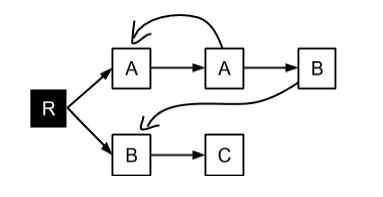
\includegraphics[width=0.8\textwidth]{figures/Example_DFA.png}
\caption{A DFA representing a set of patterns {AAB, BC}}
\label{dfa}
\end{figure}

\subsection{Construction of DFA}
\label{sec:dfa_const}
Each node consists of a character is represents, a flag signifying whether or not it is a dictionary node, and a set of the patterns it represents.\\
A dictionary node is a special kind of node which marks the end of a pattern or more, and those patterns are stored in the set of patterns it represents. \\

\begin{enumerate}
\item Forward Edge: Connecting a node representing character at position i in pattern p to the one representing the character at position i+1 in the same pattern.
\item Reverse Edge: Connecting a node to another node representing the same value in a higher level (closer to the root) provided they have the same value parents, which is insured during the building.
\end{enumerate}

\subsubsection{Setting Up the Nodes and Forward Edges}
\begin{enumerate}

\item First a root node is created and set to be the current node. The first pattern is selecter and a pointer is set to point to the first character in it.

\item If the current node does not have a forward edge to a node representing the current character, then such a node is created and a forward edge connects the current node to it. The new node becomes the the current node.

\item If the current node has a forward edge to a node representing the current character, then that node becomes the current node.

\item The pointer in the pattern moves to the next character

\item If there are no more characters in the pattern, mark the node as dictionary node with the corresponding pattern, then select the next pattern in the list and make the pointer point to the first character in it. Set the current node to the root and repeat steps 2 through 5 until there are no more patterns in the list.
\end{enumerate}

\subsubsection{Setting Up the Reverse Edges}

Expanding a node means dequeuing it and enqueuing its child nodes.
\begin{enumerate}
\item Start from the node and expand it into its children, put the child nodes into a queue.

\item Point the reverse edges of the children of the root back to the root.

\item Expand the node at the front of the queue.

\item For each node x of the children of the newly expanded node do the following:

\begin{enumerate}
        \item Set the parent of the newly expanded node as the current node.

        \item If the current node has a child node with the same value as node x, point x's reverse edge to that child, and if this child node happens to be a dictionary node for pattern p, mark node x as a dictionary of the same patter p. 
	\item If this child node does not have the same value as node x, check that it is the root, and if so, point x's reverse edge to it. Otherwise go to the node pointed to by the reverse edge of the current node set it as the current node and repeat 4.b and 4.c.
\end{enumerate}
\end{enumerate}

\subsubsection{Searching}
The search algorithm outputs any patterns it find.\\
input: string of length n.\\
\begin{enumerate}
\item set the current node to root node
\item for every character c of the input string:\\
\begin{enumerate}
\item if the current node has a forward edge pointing to a node x with the value of c, set the current node to be node x. 
\item if there is not such a forward edge, then if the current node is not the root, set the node pointed to by the reverse edge as the current node and repeat step 2.a. if the current node is the root, skip the rest of this step and step 2.c,   
\item If the current node is a dictionary node, output the patterns it represents.
\end{enumerate}
\end{enumerate}

\subsection{Theoretical Analysis}
k = total length of all patterns.\\
n = number of characters in input string\\
z = pattern occurrences in the text\\

\subsubsection{Preprocessing}
Preprocessing is done in two steps:
A Deterministic Finite Automaton (DFA) is built according to the patterns as described in the previous section. Setting up nodes and creating forward edges requires k time.\\
Traversing the DFA to add the reverse edges involves going forward k times and going up the reverse edges of a number of nodes. This number is bounded by the k, the total length of patterns since in the worst case a node at the end of each pattern will point back to the root. This gives a total of 2k for this step. \\
Hence, the preprocessing yields a runtime of 3*k = O(k). 

\subsubsection{Searching}
Each character in the input text must be compared to the content of a node once, therefore a minimum of n computations is needed for comparisons, while outputting a pattern set of a dictionary node takes constant time. However, since pattern sets are output whenever they are found in the text, then the number of times the algorithm outputs a pattern, must be taken into consideration. The worst case is when patterns are found at virtually every position of the input string. For example, let the set of patterns be $\left\{a, a^2, ..., a^m\right\}$ where m is the length of the longest pattern, and let the text by $a^n$, such that $a^i$ is i a's.\\
 
When n = 1, A(1) outputs $\left\{a\right\}$, the result of the first node.\\
When n = 2, A(2) = $\left\{a\right\}$ + $\left\{a, a^2\right\}$ = A(1) + $\left\{a, a^2\right\}$.\\
Assume that when n = i, then A(i) =  $\left\{a\right\}$+ $\left\{a, a^2\right\}$ + ... + $\left\{a, a^2, ..., a^i\right\}$.\\
Then when n = i+1, A(i+1) = $\left\{a\right\}$ + $\left\{a, a^2\right\}$ +... + $\left\{a, a^2, ..., a^i\right\}$ + $\left\{a, a^2, ..., a^i, a^(i+1)\right\}$ which can be rewritten as 
A(i+1) = A(i) + $\left\{a, a^2, ..., a^i, a^(i+1)\right\}$ \\

This shows that in the worst case, the number of pattern occurrences in the text, denoted as z, is the dominating factor in the time complexity, yeilding O(n+z).





\newpage
\section{Suffix-tree Pattern Matching}
As the third part of our comparative study, we propose a pattern matching algorithm that relies on so called suffix tree data structure. Suffix tree is a well known data structure which is commonly used in industrial and scientific applications of pattern matching today. Being a concise representation of a text composed over a finite alphabet, suffix tree, or more general suffix automaton, is a common way to compress large amounts of textual information, and it is widely used also in databases. In our study, we will perform tests of suffix tree base pattern matching algorithm, and compare it against the aforementioned Boyer-More and Aho-Corasick algorithms, trying to get an insight on when should one chose either of these algorithms.\\

Below, we will introduce first \textit{suffix trie} -- an auxillary data structure -- which we will enhance into suffix tree. Along this way, we will show that suffix tree construction algorithm is a linear time algorithm, and that suffix tree is a linear-memory data structure, following the Ukkonen's construction algorithm~\cite{ukkonen1995online}. Suffix tree construction is the preprocessing step for the pattern matching algorithm. We also, describe how to use a suffix tree of a text to find out if a pattern matches the text, and show that procedure also takes pattern length linear time.

\subsection{Suffix Trie}
Being able to consider suffix tries, and following~\cite{ukkonen1995online}, we first introduce the notations. Let text T be a string $T = t_1 t_2 \dots t_n$ over an alphabet $\Sigma$; $T_i = t_i \dots t_n$ where $1 \leq i \leq n+1$ is a suffix of the text; lets also assume that $T_{n+1} = \varepsilon$, i.e. the empty suffix. Lets denote the set of all the suffixes of the text T by $\sigma(T)$. We name the following set of objects a \textit{suffix trie} of a text T

\begin{equation}
STrie(T) = \left\{Q \cup \{\perp\}, root, F, g, f \right\}
\end{equation}

which is a deterministic finite-state automaton (DFA) which has a tree-shaped transition graph representing the trie for $\sigma(T)$. It is augmented with so called \textit{suffix function} $f$ and with an auxiliary state $\perp$. In the presented notations, the set $Q$ is the set of all the states of $STrie(T)$, which could be put into one-to-one correspondence with the substrings of $T$, i.e. with all such $x$ that $T = a\ x\ v$, where $a$ is some prefix of $T$, and $v$ is some suffix of $T$. The initial state $root$ corresponds to the empty string $\varepsilon$, and the set of final states $F$ corresponds to all the suffixes $\sigma(T)$. Finally, the transition function $g$ is defined as $g(\bar{x}, a) = \bar{y}$ for all $\bar{x}, \bar{y} \in Q$ such that $y = xa$, where $a \in \Sigma$; $g(\perp, a) = root$ for all $a \in \Sigma$.\\

Now, the suffix function $f$ is defined for each state $\bar{x} \in Q$ as follows. If $\bar{x}$ is not $root$, then $x = az$ for some $a \in \Sigma$, and we set $f(\bar{x}) = \bar{z}$. If it is $root$, $f(root) = \perp$.\\

To on-line construct a suffix trie reading a text $T$ from left to right symbol by symbol, we can apply the following simple algorithm. Suppose, we have already read some prefix of the text $T^i = t_1 \dots t_i$, and have already constructed a $STrie(T^i)$. Now, we read the next symbol $t_{i+1}$ from the text, and we need to add it to the structure and obtain $STrie(T^{i+1})$. One can notice, that all the new suffixes of $T^{i+1}$ could be obtained by concatenation of $t_{i+1}$ symbol to all the previous suffixes, i.e.

$$
\sigma(T^{i+1}) = \sigma(T^i)t_i \cup \varepsilon.
$$


\begin{enumerate}
  \item 
\end{enumerate}


\subsection{Suffix Tree}

The suffix tree for the string $S$ of length $n$ is defined as a tree such that:
\begin{itemize}
  \item The tree has exactly $n$ leaves numbered from 1 to $n$.
  \item Except for the root, every internal node has at least two children.
  \item Each edge is labeled with a non-empty substring of $S$.
  \item No two edges starting out of a node can have string-labels beginning with the same character.
  \item  The string obtained by concatenating all the string-labels found on the path from the root to leaf $i$ spells out suffix $S[i..n]$, for $i$ from 1 to n.
\end{itemize}

\subsection{definitions of some notations}
For a text, let $T = t_1t_2...t_3$ be a string over an alphabet $\Sigma$. And each string $T_i = t_it_{i+1}...t_n$ where $1 \leq i \leq n+1$ is a $suffix$ of string $T$. In particular, $T_{n+1} = \varepsilon$ is the $empty$ suffix. We define suffix tree $STree(T)$ of $T$ to be a data structure that represents $STre(T)$ in space linear in the length $|T|$ of $T$. And we denote it as $STree(T) =$
$(Q^{'}$ 
$\cup$
$\{\bot\},$
$root, g^{'}, f^{'})$.Set $Q^{'}$ consists of all branching states (states from which there
are at least two transitions) and all leaves (states from which there are no transitions) of $STrie(T)$. By definition, $root$ is included in the branching states.
The other states of $STrie(T)$ (the states other than $root$ and $\bot$ from which
there is exactly one transition) are called implicit states as states of $STree(T)$; they
are not explicitly present in $STree(T)$. Here $\bot$ is an auxiliary state.

\bibliography{references}
\nocite{*}

\end{document}
